\documentclass[12pt,a4paper]{article}
\usepackage[polish]{babel}
\usepackage[T1]{fontenc}
\usepackage{hyperref}
\usepackage{url}
\usepackage{graphicx}
\graphicspath{ {images/} }
\usepackage{csquotes}
\usepackage[utf8x]{inputenc}
\usepackage{fancyvrb}

\addtolength{\hoffset}{-1.5cm}
\addtolength{\marginparwidth}{-1.5cm}
\addtolength{\textwidth}{3cm}
\addtolength{\voffset}{-1cm}
\addtolength{\textheight}{2.5cm}
\setlength{\topmargin}{0cm}
\usepackage{algorithm}
\usepackage[noend]{algpseudocode}
\setlength{\headheight}{0cm}

\begin{document}
    \begin{titlepage}
       \begin{center}
           \vspace*{1cm}
           
           {\fontsize{23}{25}\selectfont Dokumentacja projektu\\Weather App\\Mobilne interfejsy multimedialne}
            \vspace{0.4cm}
            
            {\fontsize{17}{18}\selectfont Dawid Bitner}
           
            {\fontsize{12}{13}\selectfont 27 marca 2020}
           
            \vfill
            \vspace{0.8cm}
     
            {\fontsize{13}{14}\selectfont Politechnika Śląska\\Wydział Matematyki Stosowanej\\Rok akademicki 2019/2020}
     
       \end{center}
    \end{titlepage}
	\newpage
	\tableofcontents
	\newpage
	\section{Narzędzia, skrypty, źródła zewnętrzne}
	Do realizacji projektu użyłem jako środowiska programistycznego\textit{ Android Studio} w wersji \textit{3.5.1}. \\
    Postanowiłem, że użyję frameworka do języka \textit{Dart} - \textit{Flutter'a} w wersji \textit{v1.12.13+hotfix.8}. \\
	Emulator symulował urządzenie \textit{Nexus 5X}, na którym był zainstalowany system\textit{ Android} w wersji \textit{8.1 API 27}. \\
    \\
    Podczas realizacji projektu użyłem kilku zależności dodanych do projektu we Flutterze - opiszę je krótko na podstawie pliku \textit{pubspec.yaml} \\
    \begin{itemize}
    \begin{verbatim}
    name: weatherapp
description: Simply aplication using Open Weather Map API

version: 1.0.0+1

environment:
  sdk: ">=2.1.0 <3.0.0"

dependencies:
  flutter:
    sdk: flutter
  cupertino_icons: ^0.1.2
  retrofit: ^1.3.1
  flutter_simple_dependency_injection: ^1.0.2
  json_serializable: ^3.2.5
  bloc_pattern: ^2.5.1
  rxdart: ^0.23.1
  fluttertoast: ^3.1.3
  intl: ^0.16.1

dev_dependencies:
  flutter_test:
    sdk: flutter
  retrofit_generator: ^1.3.1
  build_runner: ^1.7.4

flutter:
  uses-material-design: true
  assets:
    - assets/
    
    \end{verbatim}
    \end{itemize}
    
    \newpage
    
    \textbf{cupertino-icons} - jest to repozytorium zasobów zawierające domyślny zestaw zasobów ikon używanych przez Flutter - wykorzystałem ikonę lupy do wyszukiwania miasta. \\ \\
    \textbf{retrofit} - wykorzystany w celu łatwego dostępu do API, bez pisania dużej ilości kodu, doskonale współgra z serializatorem i deserializatorem \textit{JSON}. \\ \\
    \textbf{flutter-simple-dependency-injection} - dzięki temu mogłem wykorzystać wstrzykiwanie zależności w swoich programie. \\ \\
    \textbf{json-serializable} - wykorzystany w celu serializacji danych, ułatwia pisanie programu poprzez tworzenie plików, przy użyciu komendy na podstawie prostych zależności zostały stworzone pliki \textit{g.dart} dzięki który można było pobierać dane z API. Przykład: \\ \\
    plik weather.dart:
    \begin{verbatim}
    import 'package:json_annotation/json_annotation.dart';

part 'weather.g.dart';

@JsonSerializable()
class Weather {
  String main;
  String description;
  String icon;
  Weather({this.main, this.description, this.icon});

  //https://flutter.dev/docs/development/data-and-backend/json
  factory Weather.fromJson(Map<String, dynamic> json) => _$WeatherFromJson(json);
  Map<String, dynamic> toJson() => _$WeatherToJson(this);
}

    \end{verbatim}
Oraz stworzony na jego podstawie plik weather.g.dart:
\begin{verbatim}
// GENERATED CODE - DO NOT MODIFY BY HAND

part of 'weather.dart';

// **************************************************************************
// JsonSerializableGenerator
// **************************************************************************

Weather _$WeatherFromJson(Map<String, dynamic> json) {
  return Weather(
    main: json['main'] as String,
    description: json['description'] as String,
    icon: json['icon'] as String,
  );
}

Map<String, dynamic> _$WeatherToJson(Weather instance) => <String, dynamic>{
      'main': instance.main,
      'description': instance.description,
      'icon': instance.icon,
    };

\end{verbatim}

\textbf{bloc-pattern} - w celu prostszego zastosowania logiki biznesowej w projekcie \\ \\
\textbf{rxdart} - w celu wykorzystania programowania reaktywnego 
\textbf{fluttertoast} - dołączone standardowo - w celu używania wyskakujących powiadomień - \textit{Toastów}. \\ \\
\textbf{intl} - ten pakiet zapewnia funkcje internacjonalizacji i lokalizacji, w tym tłumaczenie wiadomości, liczbę mnogą i płcie, formatowanie i analizę dat / liczb oraz tekst dwukierunkowy. Dołączany standardowo. \\ \\
\textbf{uses-material-design} - w celu używania \textit{Google Design}.
    
	\section{Problemy podczas realizacji}
Nie miałem większych problemów podczas realizacji tego projektu we Flutterze którego dopiero poznaję, więc stosowałem się do zaleceń przedstawianych np. na\textit{ Stack Overflow}, czy posiłkując się opinią znajomych z doświadczeniem w tej technologii. Posiłkowałem się również poradnikami zamieszczonymi pod tym adresem: \\ \url{https://bloclibrary.dev/#/?id=examples} \\
Jedyne problemy jakie wystąpiły to te związane z designem aplikacji, pierwszy raz spotkałem się z taką strukturą budowania UI.
	
    \newpage
    
	\section{Główna część projektu}
Jako stronę powitalną mamy do użytku wyszukiwarkę pogody po nazwie miasta: \\
    \begin{center}
        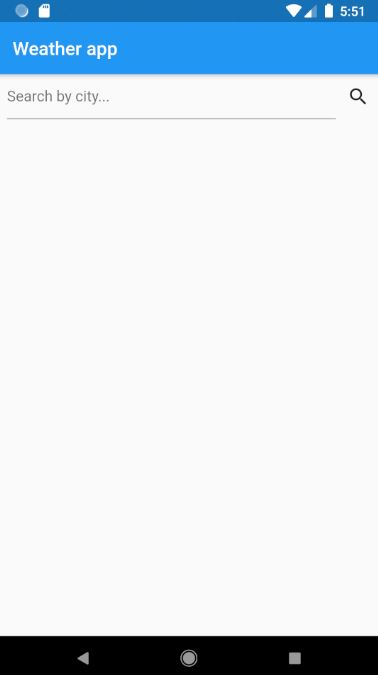
\includegraphics{1.JPG}
        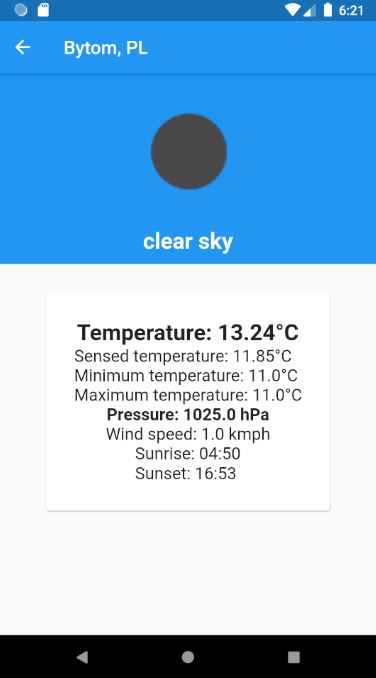
\includegraphics{2.JPG}
            \begin{scriptsize}
           Dwie karty dostępne w aplikacji
            \end{scriptsize}
    \end{center}
    Po wyszukaniu miasta zostajemy przenoszeni do części aplikacji która wyświetla informacje o pogodzie w wybranym mieście. Dostępne informacje to: nazwa miasta, kraj, ikona aktualnej pogody (zgodna z ikonami udostępnianymi przez API), opis słowny aktualnej pogody, temperatury: nominalna, odczuwalna, minimalna i maksymalna na dany dzień, ciśnienie, prędkość wiatru, oraz wschód i zachód słońca.
	\section{Opinia}
W mojej opinii pomimo prostoty projektu mogłem nauczyć się dzięki niemu wielu aspektów tworzenia aplikacji we Flutterze. Użyłem wielu popularnych i używanych komercyjnie zależności. Skorzystałem z poradników i pomocy innych osób, największe problemy sprawiało mi graficzne ułożenie interfejsu, ponieważ struktura i sposób tworzenia UI jest dla mnie mało przejrzysty, możliwe że istnieją narzędzia wspomagające programistę w tym zakresie, których jeszcze nie poznałem.

\end{document}
